\documentclass{journal}
\usepackage{graphicx}	% package for using graphics
\usepackage{float}	% package for positioning figure
\usepackage{wrapfig}	% package for wrapping figure

\title{Airframe Aerodynamic Design}

\author{Nathan Pettit}


\begin{document}
	
	\maketitle	
	
	\section{Introduction}
	
	This report covers the work done in learning how to optimize an airframe with specific parameters, using techniques and knowledge learned previously. The goal was to design an airframe that can lift 0.5 kilograms, has a wingspan no greater than 1.5 meters, and is stable.
	
	\section{Methods}
	The results of this research came from evaluating potential airframe solutions using VortexLattice.jl, as well as writing new functions to help in optimizing the airframe design. There were 4 functions that were  used:
	
	\begin{enumerate}
		\item optimize\_airframe() - this was the main function that optimized the airframe so that it met the specified requirements and was the most efficient; it employed the use of all the other functions in order to find the optimized airframe
		\item wing\_efficiency() - this calculated the inviscid span efficiency of a given airframe
		\item compare\_designs() - this plotted the important characteristics of the ideal airframe against other designs for comparison.
		\item vortex\_lattice() - this was the function that performed all the necessary VortexLattice calculations for the other functions 
	\end{enumerate}

	In order to optimize the airframe, the process, discussed in the introduction to "Engineering Design Optimization" by Joaquim R.R.A. Martins and Andrew Ning, was followed. The objective function  that was minimized was the equation used to calculate the velocity needed to produce the necessary lift to carry 0.5 kilograms (see equation \ref{eqn:needed-velocity}).
	
	\begin{equation}
		V = \sqrt{\frac{L}{(0.5)(C_L)(\rho)(S_{ref})}}
		\label{eqn:needed-velocity}
	\end{equation}

	\begin{itemize}
		\item \(L\) - the lift needed to takeoff with 0.5 kilograms, in this case 4.905 N
		\item \(\rho\) - the density of the air (1.225 \(kg/m^3\))
		\item \(S_{ref}\) - the reference area, in this case the wing area
	\end{itemize}
	
	The design variables that were altered in order to minimize that function was the mean aerodynamic chord length of the wing and the length from wing to tail on the airframe. The reason I chose these design variables was because I knew that the airframe that would generate the most lift would have the max wingspan possible (so in this case 1.5 m), and so altering the chord length would help me find the wing that needed the least speed to takeoff. I also chose the length from wing to tail as a design variable because I knew altering it would change how stable the airframe was. However, as I worked with these design variables, it was discovered that the greater the length from wing to tail, the more stable the airframe. For this reason, I put an upper limit on that length to be 2.0 m, so that the found airframe would be realistic. The way that I found the optimal airframe was I changed those design variables together, so that it found the airframe that took off at the least velocity, but was the most stable. This means that there are other configurations of the airframe where the takeoff velocity is less, but they aren't more ideal because they are less stable. The inviscid span efficiency was also evaluated using different wing tapers, in order the maximize efficiency.
		
	\section{Results and Discussion}
	
	After running the optimize\_airframe() function, it found that the most optimized airframe was one that had the following characteristics:
	
	\begin{itemize}
		\item span length = 1.5 meters
		\item mean aerodynamic chord length = 0.4111 meters
		\item length from wing to tail = 2.0 meters
		\item taper = 1.0
		\item lift coefficient = 0.06619075753338803
		\item velocity needed to produce necessary lift = 14.006916728142778 m/s
	\end{itemize}

	The aforementioned necessary lift was 4.905 Newtons. This number was found by multiplying 0.5 kilograms by 9.81 \(m/s^2\), which is the acceleration due to gravity. It is also important to note that the optimize\_airframe() function accounts for stability and makes sure that the airframe is the most stable, and so this airframe is the most stable one under the given constraints. In order to show that this airframe has been optimized, other airframes have been evaluated in order to show correctness.\\
	
	\subsection{Altered Mean Chord Length}

	When evaluating an airframe that has a mean chord length that is less than 0.411 m (I used 0.2 m for comparison), it was found that the velocity needed to generate the necessary lift was 16.942465583585317 m/s, which is greater than than the velocity needed for the optimized airframe. This shows that airframes with smaller mean chord lengths are not more optimized, as they need a greater velocity to lift the 0.5 kilograms.\\
	
	When evaluating an airframe that has a mean chord length that is greater than 0.411 m (I used 0.6 m for comparison), it was found that the velocity needed to generate the necessary lift was 12.950924026610165 m/s. It may seem that since the velocity needed is less than that of the optimized airframe, an airframe with a greater mean chord length is more optimal. Upon further inspection, this airframe is also stable. However, the yaw stability derivative(\(C_{nb}\)), is greater for the previously found optimized airframe, which means that it is more stable. This shows that as the mean chord length becomes greater, the airframe becomes less stable.\\
	
	A plot showing the lift coefficient vs. angle of attack for these 3 designs is given (see figure \ref{fig:chords}).
	
	\begin{figure}[H]
		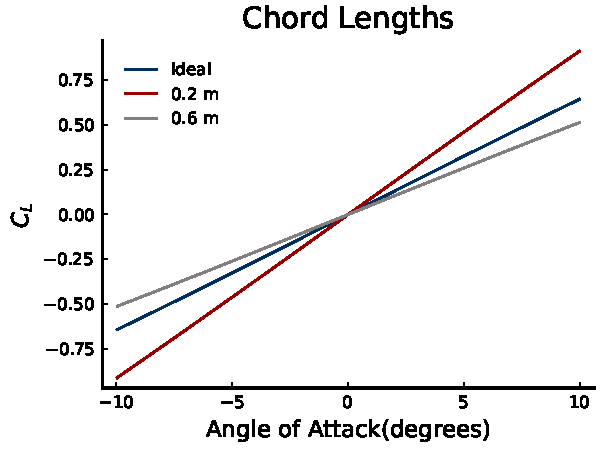
\includegraphics{../graphics/chord_lengths.pdf}
		\caption{\emph{This figure shows the lift coefficients for varying angles of attack for the 3 designs evaluated using different mean chord lengths}}
		\label{fig:chords}
	\end{figure}
	
	\subsection{Altered Length from Wing to Tail}
	
	When evaluating an airframe that has a length from wing to tail that is less than 2.0 m (I used 1.0 m), it was found that the velocity needed to generate the necessary lift doesn't change. However, the airframe is less stable as the yaw stability derivative(\(C_{nb}\)) is less than the yaw stability derivative for the optimized airframe. Therefore, as the length from wing to tail is decreased, the airframe becomes less stable.
	
	\subsection{Altered Wing Taper}
	The wing taper ratio of an airframe is found using equation \ref{eqn:taper-ratio}.
	
	\begin{equation}
		Taper\ Ratio = \frac{tip\ chord\ length}{base\ chord\ length}
		\label{eqn:taper-ratio}
	\end{equation}
	
	When evaluating an airframe that has wing taper ratio that is less 1.0 (I used 0.5), it was found that the velocity needed to calculate the necessary lift was 14.968713705560383 m/s. While this is very close to the velocity needed for the optimized airframe, it is still larger; therefore, it is not as optimal. This shows that as the wing taper ratio is decreased, the velocity needed to lift 0.5 kilograms increases, making it sub-optimal.\\
	
	A plot showing the lift coefficient vs. angle of attack for these 2 designs is given (see figure \ref{fig:taper}).
	
	\begin{figure}[H]
		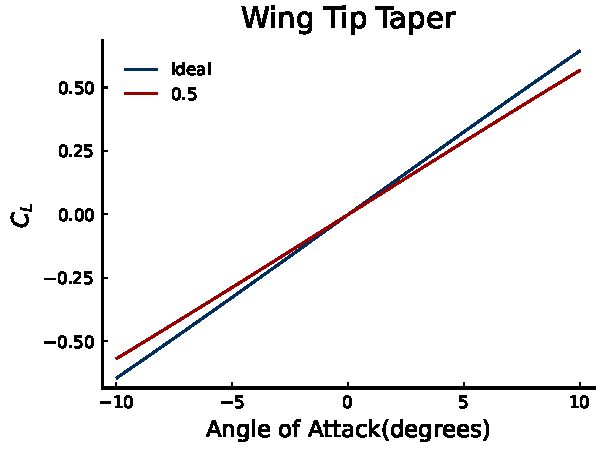
\includegraphics{../graphics/taper.pdf}
		\caption{\emph{This figure shows the lift coefficients for varying angles of attack for the 2 designs evaluated using different wing tip tapers}}
		\label{fig:taper}
	\end{figure}
	\newpage
	
	\section{Appendix}
	
	\begin{itemize}
	
		\item Engineering Design - an iterative process that engineers follow to
		develop a product that accomplishes a given task (see figure \ref{fig:design-process}).
		
		\begin{figure}[H]
			\centering
			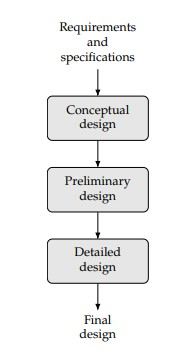
\includegraphics[scale=0.75]{../graphics/design_process}
			\caption{\emph{This figure shows the steps of the engineering design process.}}
			\label{fig:design-process}
		\end{figure}
	
		\item Design Optimization Process - s a tool that can replace an iterative design
		process to accelerate the design cycle and obtain better results (see figure \ref{fig:optimization}).
		
		\begin{figure}[H]
			\centering
			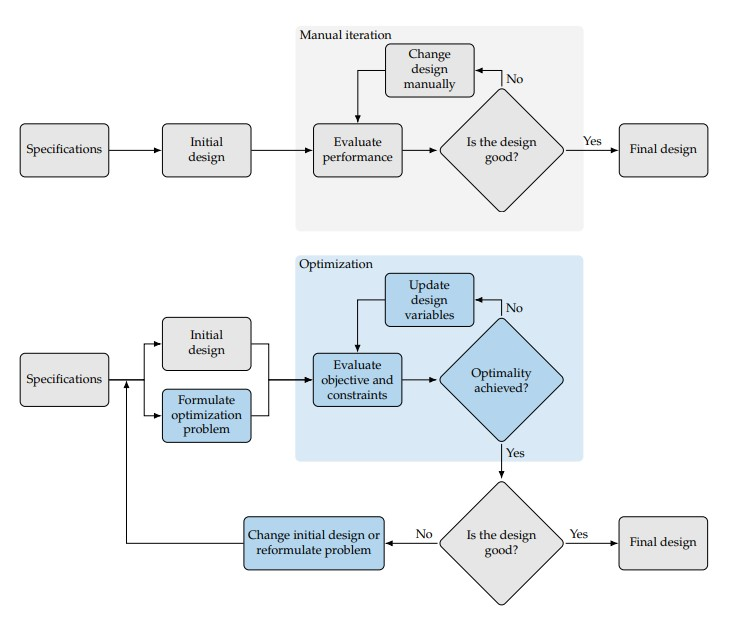
\includegraphics[scale=0.5]{../graphics/optimization_process}
			\caption{\emph{This figure shows the steps of the engineering design optimization process.}}
			\label{fig:optimization}
		\end{figure}
	
		\item Objective Function - the design optimization process requires the designer to translate their intent to a mathematical statement that can then be solved by an optimization algorithm
		\item Design Variables - the variables that describe the system, must not depend on each other or any other parameter
	\end{itemize}
	
	
\end{document}
